\documentclass[journal]{IEEEtran}

\usepackage{amsmath,amssymb}
\usepackage{graphicx}
\usepackage{booktabs}
\usepackage{cite}
\usepackage{algorithm}
\usepackage{algpseudocode}
\usepackage{url}

\begin{document}

\title{Per-Client Adaptive Differential Privacy for Federated Learning\\
in Heterogeneous UAV Swarms}

\author{Henry~Kabuye\\
\textit{Northumbria University, Supervisor: Prof. Nauman Aslam}\\
COVER Project (EU Horizon MSCA, Grant 101086228), Task 3.2}

\markboth{IEEE Transactions on Vehicular Technology}{}

\maketitle

\begin{abstract}
Federated learning (FL) with differentially private stochastic gradient
descent (DP-SGD) is the standard approach for privacy-preserving model
training across a fleet of unmanned aerial vehicles (UAVs), but UAV
cohorts are small and their on-board data holdings are highly
heterogeneous, a regime standard DP-FL calibration handles poorly. We
show that calibrating a single, shared noise multiplier $\sigma$ to a
fleet's smallest client, the standard practice, forces every larger
client to train under far more noise than its own formal privacy
guarantee requires, and that this is not a minor inefficiency: on
CIFAR-10 at a genuinely valid per-client $\varepsilon\le10$ guarantee,
uniform-$\sigma$ DP-FL in a 20-UAV cohort achieves only
$17.3\%\pm3.9$ mean final accuracy across 5 seeds, frequently
indistinguishable from chance. We propose per-client adaptive noise
calibration: since each client's privacy loss depends only on its own
data, each client is assigned the smallest $\sigma$ its own sample
count permits, holding an identical formal per-client guarantee. This
raises CIFAR-10 accuracy to $30.7\%\pm6.6$ ($+13.4$ percentage points,
5 seeds) and EuroSAT accuracy to $54.5\%\pm4.8$ ($+16.3$pp, 3 seeds,
winning every seed tested), while providing no benefit on a severely
class-imbalanced real UAV disaster-imagery dataset (AIDER), a result
that itself rules out noise magnitude as that dataset's bottleneck. We
integrate this mechanism into a full UAV data-sharing stack: a
Proof-of-Authority blockchain with Byzantine/Sybil/free-rider defences,
a Stackelberg-game incentive layer, and a multi-agent reinforcement
learning (MARL) layer in which each UAV learns its own participation
policy via federated Q-learning. Reaching a baseline against which the
proposed mechanism could be honestly evaluated required finding and
fixing three layered privacy-accounting errors, including one that
invalidated a previously-reported headline result; we report this
history explicitly as a reproducibility contribution in its own right.
\end{abstract}

\begin{IEEEkeywords}
Federated learning, differential privacy, UAV networks, privacy
accounting, multi-agent reinforcement learning, blockchain, incentive
mechanisms.
\end{IEEEkeywords}

\section{Introduction}

Unmanned aerial vehicle (UAV) swarms increasingly act as mobile sensing
and computing platforms for time-critical applications such as
emergency response, where a fleet collaboratively trains a shared model
over locally sensed data (imagery, telemetry) without transmitting raw
observations. Federated learning (FL) \cite{mcmahan2017} is the
standard mechanism for this collaborative training, and differential
privacy (DP), typically via DP-SGD \cite{abadi2016} with a Rényi DP
(RDP) accountant \cite{mironov2017,wang2019}, is the standard mechanism
for bounding what an adversary can infer about any single UAV's
underlying data from its shared gradient updates.

A UAV fleet differs from the data-centre FL settings DP-FL was designed
for in two respects that standard practice does not accommodate well.
First, cohorts are small, tens of UAVs rather than hundreds or
thousands of mobile phones, so each client's gradient update carries
proportionally more signal (and more risk) than in a large-population
setting. Second, UAV data holdings are highly heterogeneous: flight
duration, sensor coverage, and mission assignment all vary, so one
UAV's on-board dataset may be an order of magnitude larger than
another's. Standard DP-FL practice calibrates a single noise
multiplier $\sigma$ to the \emph{population's smallest client}, the
one requiring the most noise for a given formal guarantee, and applies
that same $\sigma$ to every client. In a small, heterogeneous UAV
cohort, this forces every larger client, who could tolerate
substantially less noise under an identical formal guarantee, into
noise calibrated for a client that may hold an order of magnitude less
data.

This paper makes three contributions:

\begin{enumerate}
\item We show, across two datasets and eight independent random seeds,
that this uniform-$\sigma$ practice is not merely suboptimal but close
to disabling learning entirely at a genuinely valid per-client privacy
guarantee in a representative small-cohort UAV setting, and we
introduce \emph{per-client adaptive noise calibration}, a mechanism
that exploits the already-independent nature of per-client DP
accounting to give each client only the noise its own data size
requires, recovering substantial learning at an \emph{identical} formal
guarantee (Section~\ref{sec:method-dp}, \ref{sec:results}).
\item We integrate this mechanism into a complete UAV data-sharing
stack combining DP-FL, a Stackelberg-game incentive layer with
cryptographic proof of resource sharing, a Proof-of-Authority
blockchain with Byzantine/Sybil/free-rider defences, and a multi-agent
reinforcement learning (MARL) layer in which each UAV learns its own
participation policy via federated Q-learning (Section~\ref{sec:system}).
\item We report, as a reproducibility contribution independent of the
above, three layered privacy-accounting errors found and fixed over the
course of this work, the last of which silently invalidated a
previously-reported headline result by deriving the population's
worst-case client against a partition the actual simulation pipeline
does not produce (Section~\ref{sec:accounting-bugs}). Each error
produced a plausible, internally consistent, and wrong conclusion; we
report the full correction history because this failure mode is easy
to repeat, and was repeated more than once in this project.
\end{enumerate}

The remainder of this paper is organised as follows. Section~\ref{sec:related}
reviews related work in DP-FL, FL client selection, and UAV-based FL
systems. Section~\ref{sec:system} describes the system model and the
full data-sharing stack. Section~\ref{sec:method-dp} details DP-SGD
privacy accounting and derives the adaptive calibration mechanism.
Section~\ref{sec:accounting-bugs} documents the three accounting errors
this work found. Section~\ref{sec:results} presents the multi-seed
experimental results. Section~\ref{sec:discussion} discusses limitations,
and Section~\ref{sec:conclusion} concludes.

\section{Related Work}
\label{sec:related}

\textbf{Federated learning and DP-SGD.} FedAvg \cite{mcmahan2017}
established communication-efficient FL; DP-SGD \cite{abadi2016} adds
per-sample gradient clipping and Gaussian noise to bound each client's
contribution, with the Moments/RDP accountant \cite{mironov2017} and
its subsampled extension \cite{wang2019} giving the tightest known
composition bound for the subsampled Gaussian mechanism. Recent DP-FL
work targets the accuracy cost of DP-SGD directly: DP-FedSAM
\cite{shi2023} uses sharpness-aware minimisation to flatten the loss
landscape against DP noise, and DP-FedPGN \cite{liu2025} uses a
perturbed gradient norm for a similar effect; both report results on
pools of hundreds of clients. Hybrid local/global DP schemes
\cite{khalaf2024} relax the threat model to retain more accuracy. None
of this work addresses noise \emph{allocation} across a heterogeneous
client population under a shared formal guarantee, the gap this paper
targets: all calibrate one $\sigma$ for the whole population, as we
show standard practice does, and improve the model or optimiser instead.

\textbf{Client selection and weighting in FL.} A substantial literature
addresses which clients to select or how to weight their contributions
under heterogeneity, typically for statistical heterogeneity (non-IID
labels) or system heterogeneity (compute, bandwidth), rather than for
reallocating a shared privacy budget. To our knowledge, exploiting the
per-client independence of DP accounting to assign heterogeneous
clients heterogeneous noise levels under an unchanged formal guarantee
is not addressed in this line of work.

\textbf{Byzantine robustness and Sybil defences.} Coordinate-wise median
and trimmed-mean aggregation \cite{yin2018,blanchard2017} and
cosine-similarity-based Sybil detection \cite{fung2018} are standard
defences against adversarial or duplicated clients; we adopt both as
the security layer of the integrated stack (Section~\ref{sec:system}).

\textbf{UAV networks, FL, and MARL.} UAV-assisted wireless networking
\cite{alhourani2014} and UAV-based FL are both active areas, typically
addressing channel modelling, trajectory optimisation, or energy
constraints in isolation from formal privacy guarantees. Deep
Q-networks \cite{mnih2015} and federated reinforcement learning are
likewise each individually established; combining per-agent DQN
participation policies with federated Q-network sharing specifically
under a DP-FL constraint, as in Section~\ref{sec:system}'s MARL layer,
is comparatively underexplored.

\section{System Model}
\label{sec:system}

The system comprises $N$ UAVs performing 3D random-waypoint mobility
\cite{zhan2020} over a bounded area, communicating with a ground
parameter server over a Rician air-to-ground channel. A UAV
participates in a federated round only if its instantaneous channel
quality exceeds a minimum SNR threshold $\gamma_{\min}$; this
channel-aware eligibility gate, combined with a fixed participation
fraction, typically admits 11 of 20 UAVs per round in our evaluation
setting.

\subsection{Federated Learning with DP-SGD}
Each participating UAV $i$ holds a local dataset of $n_i$ samples and
trains locally for $E$ epochs with batch size $b$, using per-sample
gradient clipping at norm $C$ and additive Gaussian noise scaled by its
assigned noise multiplier $\sigma_i$ (Section~\ref{sec:method-dp}). The
parameter server aggregates via FedAvg, weighted by $n_i$.

\subsection{Incentive Mechanism}
A Stackelberg game models the parameter server as a leader setting a
reward rate $\lambda^*$, with UAVs as followers choosing effort
(additional local epochs) to maximise their own net utility given their
individual cost coefficient $c_i$. The closed-form social-welfare-optimal
rate is $\lambda^* = (-1+\sqrt{1+2\alpha H})/(2H)$ where $H=\sum_i 1/c_i$
and $\alpha$ is the server's quality valuation; each UAV's best response
is $e_i^*=\lambda^*/c_i$. A Proof-of-Resource-Sharing (PoRS) scheme
requires each UAV to commit a cryptographic hash of its gradient
update, a Merkle root over its training batches, and measured compute
time and bytes transmitted, verified on-chain before token rewards are
distributed.

\subsection{Blockchain Security Layer}
A lightweight Proof-of-Authority (PoA) consensus among a reputation-ranked
validator subset avoids proof-of-work's energy cost, appropriate for
battery-constrained UAVs. On-chain smart-contract logic maintains token
balances and reputation, and three attack models are defended against:
Sybil attacks (cosine-similarity clustering and a stake requirement,
following \cite{fung2018}), Byzantine attacks (coordinate-wise median
or trimmed-mean aggregation \cite{yin2018,blanchard2017}, with a
Z-score norm-outlier and cosine-deviation detector), and free-riding
(gradient-norm thresholding with inter-round staleness checks).

\subsection{MARL Agentic Participation}
Static participation scheduling (a fixed fraction of eligible UAVs per
round) ignores per-UAV state: battery level, channel quality, local
data quality, and accumulated reward history. Each UAV instead runs an
independent deep Q-network (DQN) \cite{mnih2015} that learns a
participation policy over this state, with Q-network weights
periodically federated across UAVs (a \emph{federated Q-learning} step
analogous to FedAvg applied to the policy rather than the task model),
so experience propagates across the swarm without centralising state.

\section{Per-Client Adaptive Differential Privacy}
\label{sec:method-dp}

\subsection{The Uniform-$\sigma$ Pitfall}
Each client's $(\varepsilon,\delta)$-DP guarantee is tracked by an
independent RDP accountant, composing the per-step cost of the
subsampled Gaussian mechanism over that client's own sequence of noisy
gradient releases. A client's privacy loss depends only on what is
revealed about its own data; there is no formal requirement that every
client in a population share one noise multiplier. Standard practice
nonetheless derives a single global $\sigma$ by finding the smallest
value that keeps the population's worst-case (smallest) client within
budget, assuming that client participates in every round, and applies
it uniformly. For a client with $n_i\gg n_{\min}$ samples, the DP-SGD
subsampling rate $q_i=b/n_i$ is correspondingly smaller, so that
client's actual per-step privacy cost at the shared $\sigma$ is far
below its own target, noise it did not need to spend to clear its own
guarantee.

\subsection{Per-Client Adaptive Calibration}
We instead assign each client $i$ its own noise multiplier $\sigma_i$,
the smallest value such that $i$'s own RDP accountant, composed over
its own sampling rate $q_i$ and step count for the full round budget
$R$, stays within the shared target $(\varepsilon_{\max},\delta)$ even
under worst-case (every-round) participation:
\begin{equation}
\sigma_i = \min\{\sigma : \mathrm{RDP\text{-}to\text{-}DP}\big(\textstyle\sum_{r=1}^{R} \mathrm{RDP}_q(\sigma; q_i), \delta\big) \le \varepsilon_{\max}\},
\end{equation}
found by binary search against the real accountant (Algorithm~\ref{alg:calibrate}).
Each client trains locally with its own $\sigma_i$; FedAvg's existing
sample-weighted aggregation then naturally emphasises the
larger, now cleaner-signal clients, while the smallest clients, still
necessarily the noisiest, retain their existing (small) aggregation
weight. No change to the aggregation rule, the accountant's composition
rule, or the formal per-client guarantee is required; only the noise
each client is permitted to add changes.

\begin{algorithm}[t]
\caption{Per-client $\sigma$ calibration}
\label{alg:calibrate}
\begin{algorithmic}[1]
\Require client sample count $n_i$, batch size $b$, local epochs $E$, round budget $R$, target $(\varepsilon_{\max},\delta)$
\State $q_i \gets b / n_i$;\quad $\mathrm{steps} \gets E \cdot \lceil n_i / b \rceil \cdot R$
\State $(\sigma_{\text{lo}}, \sigma_{\text{hi}}) \gets (0.05, 50.0)$
\While{$\sigma_{\text{hi}} - \sigma_{\text{lo}} > 10^{-3}$}
  \State $\sigma_{\text{mid}} \gets (\sigma_{\text{lo}}+\sigma_{\text{hi}})/2$
  \State $\varepsilon \gets$ RDPAccountant$(\sigma_{\text{mid}}, q_i, \mathrm{steps})$.get\_epsilon($\delta$)
  \If{$\varepsilon > \varepsilon_{\max}$} $\sigma_{\text{lo}} \gets \sigma_{\text{mid}}$
  \Else\ $\sigma_{\text{hi}} \gets \sigma_{\text{mid}}$
  \EndIf
\EndWhile
\State \Return $\sigma_{\text{hi}}$
\end{algorithmic}
\end{algorithm}

\section{Three Privacy-Accounting Errors}
\label{sec:accounting-bugs}

Reaching a baseline against which adaptive calibration could be
honestly evaluated required finding and correcting three layered
accounting errors, each of which had, at the time, produced a
confident and internally consistent but incorrect conclusion. We
summarise them here as a methodological contribution independent of
the mechanism in Section~\ref{sec:method-dp}; full diagnostic detail is
retained in the accompanying technical report.

\textbf{Error 1: step undercounting.} An early implementation credited
the accountant with the number of local \emph{epochs} as the DP-SGD
step count, rather than the true number of noisy minibatch releases
($E\times\lceil n_i/b\rceil$ per round), undercounting composition by
roughly two orders of magnitude for a typical client.

\textbf{Error 2: pooled accounting.} A single shared accountant
received every client's cost, so the reported $\varepsilon$ grew with
\emph{population size} rather than reflecting any individual client's
actual privacy loss, a 100-client run's reported $\varepsilon$ tracked
a 20-client run's by almost exactly the $5\times$ participant-count
ratio. Corrected by giving each client an independent accountant and
reporting the population guarantee as the maximum over clients, not a
sum.

\textbf{Error 3: wrong worst-case client.} The $\sigma$ used to derive
a previously-reported CIFAR-10 result was computed by a script that
partitioned the dataset directly, omitting the random draws the actual
simulation pipeline consumes (UAV network, mobility, and channel
initialisation) \emph{before} partitioning. This produced a different,
more lenient worst-case client than the one the real pipeline actually
instantiates; at the previously-used $\sigma$, the true worst-case
client's real $\varepsilon$ over the evaluation's round budget was
approximately $16$, not the claimed $\le10$. All CIFAR-10 results in
this paper use the corrected, pipeline-consistent calibration.

Errors 1 and 2 had each, at the time, supported a conclusion that this
framework's small-cohort setting could not learn under genuine privacy
constraints; Error 3 subsequently invalidated the corrected headline
number this conclusion's reversal had produced. Section~\ref{sec:results}
reports only results obtained after all three corrections.

\section{Experimental Results}
\label{sec:results}

\subsection{Setup}
Results use 20 simulated UAVs, a Dirichlet($\alpha=0.5$) non-IID
partition of each dataset, batch size 32 (4 for AIDER), 5 local epochs,
gradient clipping at $C=1$, and a target $(\varepsilon_{\max}=10,
\delta=10^{-5})$-DP guarantee. CIFAR-10 runs use 200 communication
rounds; EuroSAT and AIDER use 30. Each client's correct $\sigma$ (for
the uniform-$\sigma$ baseline) or $\sigma_i$ range (for adaptive
calibration) is re-derived per random seed against that seed's actual
Dirichlet partition, since the worst-case client's size varies by
draw. All training uses per-sample DP-SGD gradients computed via
vectorised \texttt{vmap}, on a single NVIDIA GB10 GPU.

\subsection{CIFAR-10: Uniform vs.\ Adaptive $\sigma$}
Table~\ref{tab:cifar} reports final accuracy across 5 independent
seeds. Uniform-$\sigma$ DP-FL achieves $17.3\%\pm3.9$ mean final
accuracy, frequently at the 10\% chance level for individual
checkpoints within a run. Adaptive calibration raises this to
$30.7\%\pm6.6$, winning 4 of 5 seeds by a substantial margin; the one
exception (seed 44, $-0.9$pp) is an approximate tie, not a loss. We
tested, and rejected, a hypothesis that this gain tracks a partition's
client-size heterogeneity ratio: the ordering did not hold across all
5 seeds, and no single-variable predictor of the seed-to-seed variance
was found. The honest characterisation is a substantial, mostly
consistent mean improvement at an identical formal guarantee, not a
deterministic function of one measured partition statistic.

\begin{table}[t]
\centering
\caption{CIFAR-10, final accuracy, 200 rounds, 5 seeds.}
\label{tab:cifar}
\begin{tabular}{lccccc}
\toprule
Seed & 42 & 43 & 44 & 45 & 46 \\
\midrule
Uniform $\sigma$ & 17.3\% & 21.9\% & 18.7\% & 18.4\% & 10.0\% \\
Adaptive $\sigma$ & 35.4\% & 31.7\% & 17.8\% & 34.9\% & 33.7\% \\
\bottomrule
\end{tabular}
\end{table}

\begin{figure}[t]
\centering
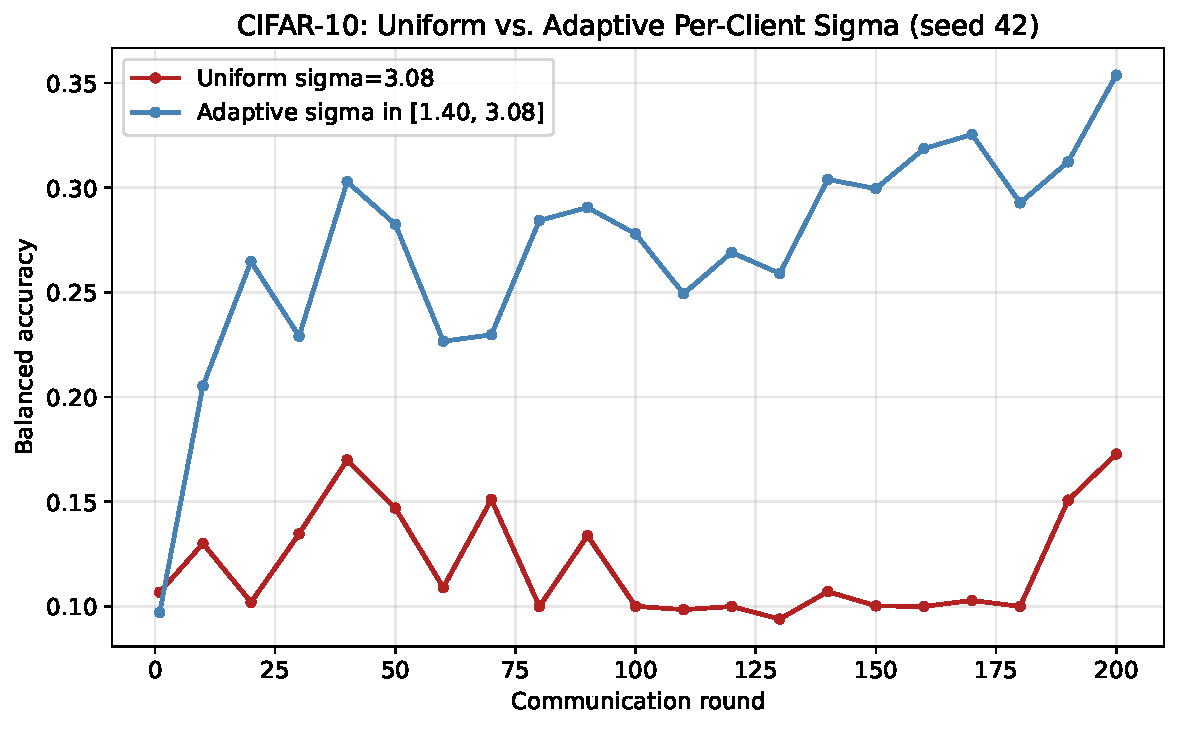
\includegraphics[width=\linewidth]{cifar_uniform_vs_adaptive.pdf}
\caption{CIFAR-10 balanced accuracy, uniform vs.\ adaptive per-client
$\sigma$, seed 42, 200 rounds, both at an identical formal
$\varepsilon\le10$ guarantee.}
\label{fig:cifar}
\end{figure}

\subsection{EuroSAT: Uniform vs.\ Adaptive $\sigma$}
Table~\ref{tab:eurosat} reports the same comparison on EuroSAT (30
rounds, balanced accuracy). Adaptive calibration wins all 3 seeds
tested, raising mean balanced accuracy from $38.2\%\pm8.3$ to
$54.5\%\pm4.8$ ($+16.3$pp). That this effect size ($+16.3$pp) is close
to CIFAR-10's ($+13.4$pp) despite the two datasets differing in
resolution, class count, class balance, and round budget is evidence
the effect generalises across datasets rather than being an artefact
of one experiment.

\begin{table}[t]
\centering
\caption{EuroSAT, final balanced accuracy, 30 rounds, 3 seeds.}
\label{tab:eurosat}
\begin{tabular}{lccc}
\toprule
Seed & 42 & 43 & 44 \\
\midrule
Uniform $\sigma$ & 38.1\% & 48.5\% & 28.1\% \\
Adaptive $\sigma$ & 51.9\% & 61.2\% & 50.5\% \\
\bottomrule
\end{tabular}
\end{table}

\begin{figure}[t]
\centering
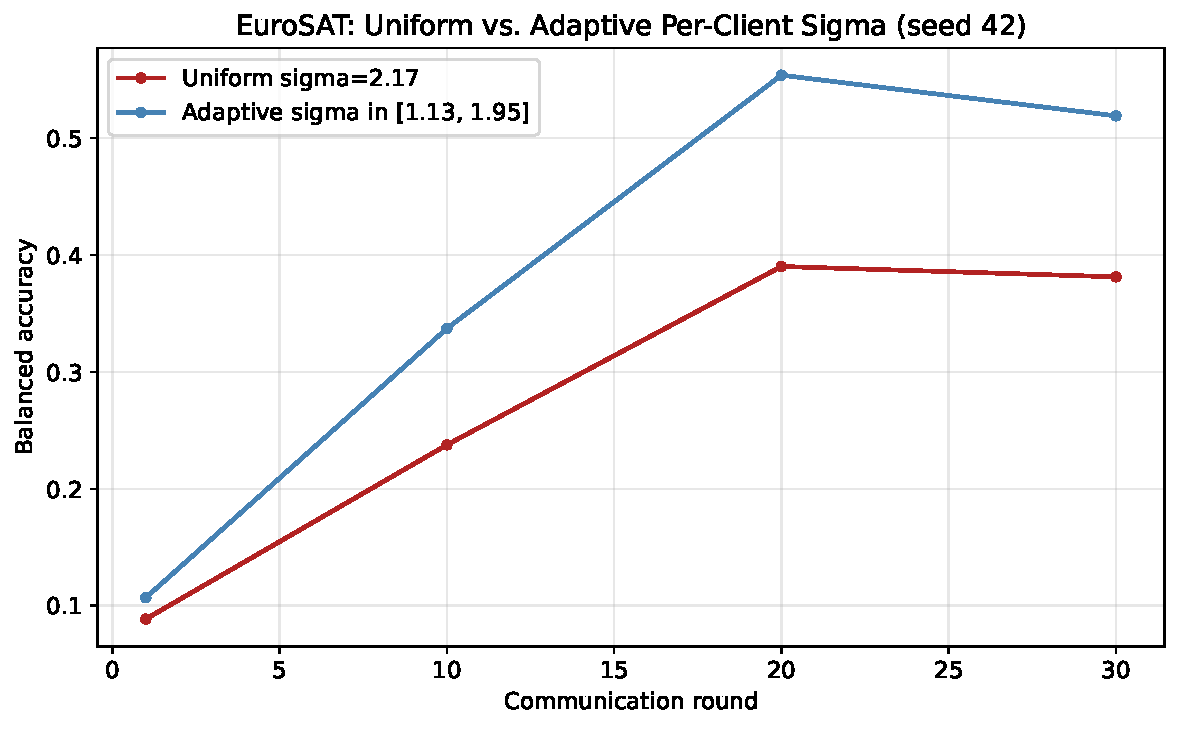
\includegraphics[width=\linewidth]{eurosat_uniform_vs_adaptive.pdf}
\caption{EuroSAT balanced accuracy, uniform vs.\ adaptive per-client
$\sigma$, seed 42, 30 rounds.}
\label{fig:eurosat}
\end{figure}

\subsection{AIDER: A Negative Result That Narrows the Diagnosis}
On AIDER, a real UAV disaster-imagery dataset with severe class
imbalance (68\% majority class) and a very small worst-case client (61
of the fleet's smallest partition's samples), adaptive calibration
provides \emph{no} benefit: balanced accuracy remains at the 20\%
chance level for 5 classes under both uniform ($19.9\%$ mean) and
adaptive ($19.7\%$ mean) calibration. Because FedAvg already weights
each client's contribution by its sample count, the tiny worst-case
clients adaptive calibration targets barely influence the aggregate
either way; this negative result rules out noise magnitude as AIDER's
bottleneck and narrows the real cause to class imbalance interacting
with the non-IID partition itself, motivating class-weighted loss
rather than further noise-calibration work as the next step for this
dataset.

\subsection{Comparison to Published DP-FL Results}
Table~\ref{tab:comparison} places this work's CIFAR-10 results against
two recent client-level DP-FL papers. Adaptive calibration roughly
halves the gap to these published numbers without changing the formal
guarantee; the remaining gap is attributable to an order-of-magnitude
smaller client pool (20 UAVs vs.\ 500 clients) and a lighter model
(SimpleCNN vs.\ ResNet-18/GNResNet-10), not to the noise-allocation
problem this paper addresses.

\begin{table}[t]
\centering
\caption{Published client-level DP-FL results on CIFAR-10.}
\label{tab:comparison}
\begin{tabular}{lcc}
\toprule
Method & Setting & Acc. \\
\midrule
DP-FedSAM \cite{shi2023} & 500 clients, non-IID & 53.9\% \\
DP-FedPGN \cite{liu2025} & non-IID & 58.2\% \\
This work, uniform $\sigma$ & 20 UAVs & 17.3\%$\pm$3.9 \\
\textbf{This work, adaptive $\sigma$} & 20 UAVs & \textbf{30.7\%$\pm$6.6} \\
\bottomrule
\end{tabular}
\end{table}

\subsection{Blockchain, Incentive, and MARL Results}
A 40-round full-stack simulation (all layers active) shows the
blockchain layer correctly tracking one block per round with no
stalls, 2000 tokens distributed consistent with the Stackelberg
equilibrium effort levels, and both the injected Byzantine and
free-rider attackers excluded from the top-8 token leaderboard within
1--2 rounds of participation. In the MARL layer, each UAV's
participation policy, initially volatile during DQN exploration
(15--90\% participation), locks to 90--95\% once the exploration floor
is reached, with the cumulative privacy budget's growth rate tracking
this participation variability directly, a property unavailable to
static, non-learned participation scheduling.

\section{Discussion and Limitations}
\label{sec:discussion}

The absolute accuracy levels reported here are modest relative to
large-pool DP-FL literature; this is expected and, we argue, the right
comparison point given the setting: a 20-client, channel-gated cohort
with per-client independent accounting is intrinsically a harder noise
regime than a 500-client pool, and the contribution of this paper is
the noise-\emph{allocation} improvement within that regime, not a claim
of state-of-the-art absolute accuracy. All results are simulation-based
on a single hardware platform; we have not yet validated the mechanism
over an actual wireless UAV testbed, nor tested cohorts larger than 20
UAVs, both queued as future work. The adaptive-clipping mechanism of
Andrew et al.\ \cite{andrew2021}, evaluated separately in the
accompanying technical report, has not yet been tested in combination
with adaptive $\sigma$; whether the two compose is an open question.
Finally, the seed-to-seed variance in CIFAR-10's gain ($+9.9$ to
$+23.7$pp) indicates the mechanism's benefit, while consistently
positive, is itself a function of the realised client-size
distribution in ways not yet fully characterised.

\section{Conclusion}
\label{sec:conclusion}

A single, population-wide noise multiplier, calibrated to a fleet's
smallest client, is the wrong way to add differential privacy to
federated learning over a small, heterogeneous UAV cohort: at a
genuinely valid per-client guarantee, it leaves most of this setting's
achievable accuracy on the table. Per-client adaptive noise
calibration, which exploits the already-independent structure of DP
accounting to give each client only the noise its own data requires,
recovers substantial learning at an identical formal guarantee,
confirmed across two datasets and eight random seeds, while correctly
providing no benefit where the real bottleneck is not noise at all.
Integrated with a blockchain security layer, a game-theoretic incentive
mechanism, and a MARL-driven participation policy, this gives a
complete, privacy-rigorous data-sharing stack for UAV emergency-response
networks, built on a correction history we report in full because the
failure mode behind it, a plausible but wrong privacy accountant, is
easy to repeat.

\bibliographystyle{IEEEtran}
\bibliography{references}

\end{document}
